\documentclass[laboratorio]{guia}

\def \practnum {11}
\def \practica {Redes de difracci\'on}

\def \materia {Laboratorio de F\'\i sica II para Qu\'\i micos}
\def \periodo {2do. Cuatrimestre de 2015}
\def \catedra {Pablo Cobelli}
\def \website {http://materias.df.uba.ar/f2qa2015c2}

\usepackage{graphics}
\usepackage{amsmath}
\usepackage{amsfonts}
\usepackage{graphicx}
\usepackage{float}
\usepackage{wrapfig}
\usepackage{subfigure}
\usepackage{bm}
\usepackage{grffile}
\usepackage{color}
\usepackage{framed}
\usepackage[utf8]{inputenc}
\usepackage[T1]{fontenc}
\usepackage{lmodern}
\usepackage{circuitikz}
\usepackage[spanish]{babel}
\usepackage{babelbib}
\selectbiblanguage{spanish}



%----------------------------------------------------------
% Agrega al path de figuras el subdirectorio con el mismo
%     nombre que el archivo principal del proyecto
\graphicspath{{./\jobname/}}

%----------------------------------------------------------
% Definicion del entorno 'sabermas'
\makeatletter
\definecolor{shadecolor}{rgb}{0.89,0.91,0.94}
\newenvironment{sabermas}[1]{%
\vfill
\begin{shaded}
  \begin{center}
  {\textsection{Para saber m\'as}}
  \end{center}
  #1
\sf } 
{%
\end{shaded}%
}
\makeatother

%----------------------------------------------------------
% Definicion del entorno 'problema'
\newcounter{ContadorProblema}
\setcounter{ContadorProblema}{0}
\newcounter{TieneFiguraAsociada}
\setcounter{TieneFiguraAsociada}{0}
\newcounter{UbicacionFigura}
\setcounter{UbicacionFigura}{0}

\newenvironment{problema}[2][]
{%
    \ifx\relax#1\relax%
        \setcounter{TieneFiguraAsociada}{0}
        \else
        \setcounter{TieneFiguraAsociada}{1}
    \fi
    \def \archivofigura {#1}
    % 
    \refstepcounter{ContadorProblema}
    \noindent%
    \ifnum\value{TieneFiguraAsociada} < 1%
        {\sffamily \bfseries Problema \arabic{ContadorProblema}.}
        %{\sc {#1}}%
        \par\nobreak\par\nobreak%
        \medskip 
    \else
        % Va con figura; resta determinar de que lado.
        \ifnum\value{UbicacionFigura} < 1
            % Poner la figura del lado derecho
            \begin{minipage}{12.25cm}
            {\sffamily \bfseries Problema \arabic{ContadorProblema}.}
            %{\sc {#1}}%
            \par\nobreak\par\nobreak%
            \medskip 
        \else
            % Poner la figura del lado izquierdo
            \begin{minipage}{4.5cm}
                \centering
                \includegraphics[width=4.5cm]{\archivofigura}
                {\footnotesize {\sffamily Esquema asociado al 
                problema \arabic{ContadorProblema}}.}
            \end{minipage}\hfill%
            \begin{minipage}{12.25cm}
                {\sffamily \bfseries Problema \arabic{ContadorProblema}.}
                %{\sc {#1}}%
                \par\nobreak\par\nobreak%
                \medskip 
        \fi
    \fi
}
{%
    \ifnum\value{TieneFiguraAsociada} < 1%
        % \par \bigskip \vskip 0.3cm
    \else
        % Va con figura; resta determinar de que lado.
        \ifnum\value{UbicacionFigura} < 1
            % Poner la figura del lado derecho
            \end{minipage}\hfill%
            \begin{minipage}{4.5cm}
                \centering
                \includegraphics[width=4.5cm]{\archivofigura}
                {\footnotesize {\sffamily Esquema asociado al 
                problema \arabic{ContadorProblema}}.}
            \end{minipage}
        \else
            % Poner la figura del lado izquierdo
            \end{minipage}%
        \fi
    \fi
    \setcounter{TieneFiguraAsociada}{0}
    \par \bigskip \vskip 0.3cm
    % Permutamos el valor de la ubicacion
    \ifnum\value{UbicacionFigura} < 1
        \setcounter{UbicacionFigura}{1}
    \else
        \setcounter{UbicacionFigura}{0}
    \fi
}

%----------------------------------------------------------
% Definicion/Redefinicion de estilos
\renewcommand{\vec}[1]{\ensuremath{\mathbf{#1}}}



\hyphenation{ coe-fi-cien-tes coe-fi-cien-te au-to-va-lor
              au-to-va-lo-res co-rres-pon-der pro-ble-ma 
              cual-quie-ra po-la-ri-za-cio-nes }

\graphicspath{{./redes/}}

\begin{document}
\objetivo{Medir el espectro de emisión de una lámpara de sodio empleando redes de difracción.
  Determinar los límites del espectro visible utilizando una fuente de luz blanca. 
  \tematicas{Redes de difracción por reflexión y transmisión, espectro de emisión.}
  }
\maketitle


\section{Redes de difracción}

Una red de difracción es una estructura repetitiva que se utiliza para introducir una perturbación periódica en un frente de onda.
Entre las configuraciones más sencillas se encuentra la red plana de transmisión; formada por una serie de rendijas idénticas y equiespaciadas. 

Si un frente de ondas plano incide sobre una red, el patrón de difracción observado sobre una pantalla alejada (difracción de Fraunhoffer) presenta una distribución de intensidad dada por
\begin{equation}
  I(\theta) = I_0 \: \left( \frac{\sin \beta}{\beta} \right)^2 \: 
  \left[ \frac{\sin N\alpha}{\sin \alpha}\right]^2,
  \label{eq:difraccion}
\end{equation}
donde 
\begin{align*}
  \alpha &= \frac{\pi b}{\lambda} \: 
  \left(\sin \theta - \sin \theta_0 \right), \\
  \beta  &= \frac{\pi a}{\lambda} \: 
  \left(\sin \theta - \sin \theta_0 \right), \\
\end{align*}
siendo \(a\) el ancho de cada rendija de la red, \(b\) el espaciado entre ellas, \(\lambda\) la longitud de onda del haz incidente, \(\theta_0\) el ángulo que forma el haz incidente con la red y \(\theta\) la posición angular del haz cuya intensidad estamos observando en la pantalla.

En la ecuación \eqref{eq:difraccion}, el factor entre paréntesis está asociado a la \emph{difracción} producida por cada rendija presente en la red.
El factor entre corchetes, por otro lado, da cuenta de la \emph{interferencia} entre las \(N\) rendijas de la red. 

Para valores específicos de \(\alpha\) y \(\beta\), la intensidad registrada \(I(\theta)\) presentará máximos principales sobre la pantalla de observación, entre los cuales observará también máximos secundarios.
El resultado de esta combinación es la interferencia \emph{modulada} por la figura de difracción.
Dado que en este caso la campana central de difracción resulta mucho más ancha que la separación entre los máximos de interferencia, los órdenes que usualmente se observan con una red corresponden a la interferencia producida por las \(N\) rendijas que componen
la red de difracción.
Si nos concentramos entonces en el factor de interferencia, encontramos que la intensidad resulta máxima cuando se verifica
\begin{equation}
  \alpha = m \pi, \quad \quad \text{siendo } m = 0, \pm 1, \pm 2, \ldots.
\end{equation}

En base a esta condición, el entero \(m\) recibe el nombre de \emph{orden de interferencia}.
Reemplazando este valor en la expresión para \(\alpha\), surge la condición
\begin{equation}
  \sin \theta_m - \sin \theta_0 = m \frac{\lambda}{b},
\end{equation}
a partir de la cual es posible determinar el ángulo \(\theta_m\) correspondiente al máximo de interferencia de orden \(m\).
Esta expresión se denomina comúnmente \emph{ecuación de la red}. 

Observe que si el haz incidente no es monocromático, la ecuación de la red sigue teniendo validez, pero constituye ahora una condición que se cumple para cada longitud de onda considerada.
Reflexione acerca de cómo es la relación entre la posición angular del máximo de interferencia y la longitud de onda de la luz considerada.
A mayor longitud de onda, ¿la desviación del haz es mayor o menor?

Analice cómo es la distribución de los máximos cuando la incidencia es normal (\(\theta_0 = 0\)) y cuando no lo es (\(\theta_0 \neq 0\)).
Verifique su análisis comparando con la figura \ref{fig:ordenes} 
\begin{figure}
  \centering
  \def\svgwidth{\columnwidth}
  \input{./redes/ordenes.pdf_tex}
  \caption{Numeración de órdenes de los máximos ante incidencia no normal.}
  \label{fig:ordenes}
\end{figure}


\section{Medición del espectro de emisión de una lámpara de sodio}

En esta práctica se medirán la(s) longitud(es) de onda emitida(s) por una lámpara de sodio (\isotope{Na}) utilizando para ello una red de transmisión y un goniómetro (instrumento que se utiliza para medir ángulos).
Se describen a continuación los pasos a seguir en esta experiencia.


\subsection{Calibración del goniómetro}
  El goniómetro consta de una platina giratoria solidaria a un limbo graduado, sobre la cual se coloca la red.
  Un colimador, para crear un haz incidente de rayos paralelos, y un anteojo que permite llevar el plano de observación al infinito, el anteojo es móvil y posee un vernier para medir el ángulo de giro sobre el limbo graduado.
  El anteojo tiene un retículo en forma de cruz que permite definir mejor las posiciones que se miden.

  Antes de medir, el dispositivo debe ser ajustado para trabajar bajo las condiciones de difracción de Fraunhofer e incidencia normal.
  Para ello debe enfocar el colimador y el anteojo.
Primero se enfoca el anteojo mirando un objeto distante (enfoque a infinito) desplazando el ocular del tubo.
  Luego se enfoca el colimador enfrentándolo al anteojo y desplazando la rendija que se halla adherida a él hasta obtener una imagen nítida de ella.

  A continuación se debe ubicar la red paralela al eje del goniómetro y aproximadamente perpendicular al haz colimado.
  La red se encuentra paralela al eje cuando la imagen de la rendija a través de la red se halle centrada y paralela al eje vertical del retículo.
  Para lograr posicionarla correctamente la platina cuenta con tres tornillos de nivelación.


\subsection{Posicionamiento de la red en el goniómetro} % (Ver Ap\'endice). 
\begin{figure}[t!]
    \centering
    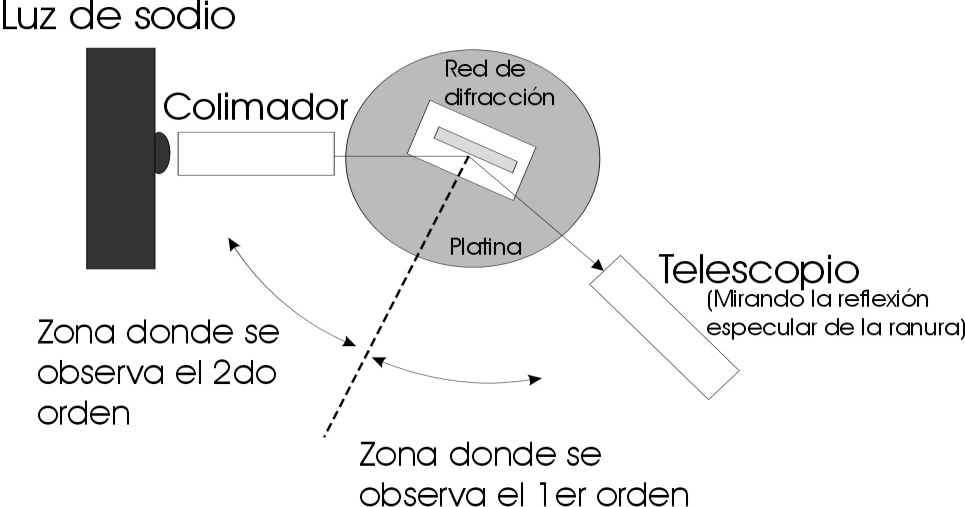
\includegraphics[width=8.5cm]{LG11--002.png}
    \caption{Esquema del dispositivo.
      Note la ubicación de la red respecto del haz proveniente de la lámpara de Na.
    }
    \label{fig:1}
\end{figure}
En la figura \ref{fig:1} se muestra el dispositivo a montar.
La red se coloca sobre la platina de modo que ésta quede perpendicular al haz incidente y centrada, es decir que el haz debe incidir en forma paralela a la normal de la red (\(\theta_0 = 0\)).
¿Por qué?
Si así no fuera, ¿qué precaución debe tomar al realizar los cálculos?
Para asegurarse incidencia normal se ubica el anteojo enfrentando al colimador y se lee la posición angular (\(L_0\)).
A continuación, se buscan los máximos correspondientes al mayor orden de interferencia visible; primero hacia un lado y luego hacia el otro, registrando los ángulos correspondientes.
Si la desviación respecto de \(L_0\) correspondiente a un mismo orden de interferencia, es idéntica hacia ambos lados se puede considerar que la red está ubicada en forma perpendicular al haz incidente.
Justifique por qué esta afirmación es válida).
Si observa que la red no está centrada, gire la platina levemente y determine nuevamente la desviación de los máximos hacia ambos lados hasta que sus observaciones coincidan.


\subsection{Mediciones}
  Conociendo la periodicidad de la red y midiendo los ángulos asociados a los  máximos de interferencia se pueden calcular las longitudes de onda emitidas por la lámpara de \isotope{Na}, a partir de la ecuación de la red.
  Mida todos los órdenes observables y construya un gráfico de \(\sin{\theta_m}\) en función de \(m\). 
  ¿Cuántas longitudes de onda espera observar?
        
        
\subsection{El doblete del sodio}
  En la lámpara de \isotope{Na} hay presentes, en realidad, dos longitudes de onda correspondientes a lo que nuestros ojos perciben como un color amarillo.
  Estas líneas de emisión son muy cercanas y no es posible resolverlas en el primer orden de interferencia. 
  ¿A partir de qué orden puede apreciar el doblete del \isotope{Na}? 
  Intente medirlo.



\section{Determinación de los límites del espectro visible}

Reemplace ahora la lámpara de \isotope{Na} por una de luz blanca y observe su espectro de emisión empleando el mismo montaje experimental que utilizó previamente.
En estas condiciones, 
\begin{enumerate}
  \item 
¿En qué aspectos difiere el espectro observado al de la lámpara de \isotope{Na}?
¿A que se debe la diferencia? 
  \item Mida las longitudes de onda asociadas a los límites que percibe.
\end{enumerate}


\section{Redes de difracción por reflexión}

Una red de reflexión es una red de difracción constituida por una serie de surcos hechos sobre una superficie metálica.
La mayoría de las redes de reflexión están construidas de forma tal que la posición del máximo de difracción es diferente de la posición del orden cero de interferencia.
De este modo se logra que la mayor intensidad de luz (asociada al máximo principal de difracción) esté dirigida hacia órdenes superiores de interferencia donde la red tiene mayor poder resolvente.
Este tipo de construcción recibe el nombre de \emph{blaze} o, en castellano, \emph{resplandor}.
Con estas redes resulta conveniente trabajar en incidencia oblicua(casi razante), a fin de poder observar mejor los distintos órdenes de interferencia. 

No obstante sus diferencias con las redes de transmisión, resulta fácil mostrar que la ecuación para este tipo de redes es idéntica a la obtenida para aquellas.
Muéstrelo. 

Dado que se trabaja con incidencia oblicua, es importante medir en forma precisa el ángulo de incidencia.
Para ello, emplearemos nuevamente el goniómetro. 

Una forma de fijar los ángulos en el goniómetro en una posición de referencia conocida consiste en colocar el ángulo cero de la platina en forma coincidente con el haz incidente.
Esto se logra observando la ranura del colimador con el telescopio, ya que en esta posición el colimador y el telescopio forman un ángulo de \(\pi\)~rad.
Mueva entonces la platina hasta hacer coincidir la marca de \SI{180}{\degree} con el cero del vernier del telescopio.
Coloque ahora la red poniendo atención a que quede centrada en la platina, y de modo tal de lograr un ángulo de incidencia no menor a \SI{65}{\degree} (¿por qué?).
Calcule, a partir de la medición del ángulo asociado al orden cero, la posición de la normal de la red.
Mida los ángulos de cada orden y cada longitud de onda.
A partir de los datos obtenidos, determine las longitudes de onda. 



% \section*{Apéndice}

% El goni\'ometro consta de una platina giratoria solidaria a un limbo graduado,
% sobre la cual se coloca la red. Un colimador, para crear un haz incidente de 
% rayos paralelos, y un anteojo que permite llevar el plano de observación al 
% infinito, el anteojo es móvil y posee un vernier para medir el ángulo de giro
% sobre el limbo graduado. El anteojo tiene un retículo en forma de cruz que 
% permite definir mejor las posiciones que se miden.

% Antes de medir, el dispositivo debe ser ajustado para trabajar bajo las 
% condiciones de difracción de Fraunhofer e incidencia normal. Para ello debe 
% enfocar el colimador y el anteojo. Primero se enfoca el anteojo mirando un 
% objeto distante (enfoque a infinito) desplazando el ocular del tubo. Luego se 
% enfoca el colimador enfrentándolo al anteojo y desplazando la rendija que se 
% halla adherida a él hasta obtener una imagen nítida de ella.

% A continuación se debe ubicar la red paralela al eje del goniómetro y 
% aproximadamente perpendicular al haz colimado. La red se encuentra paralela 
% al eje cuando la imagen de la rendija a través de la red se halle centrada 
% y paralela al eje vertical del retículo. Para lograr posicionarla 
% correctamente la platina cuenta con tres tornillos de nivelación.


%\begin{sabermas}
%Para saber mas haria falta leer un poco las siguientes referencias.
%indeed up to 90\% of the energy is in wave modes for the lower
%wavenumbers. While this results point that waves dominate the largescale
%dynamics, it is also clear that they do not govern the smaller scales.
%This puts theories in which eddies are not accounted for on.
%\end{sabermas}



\nocite{Alonso1998,Jenkins2001,Hecht1986}
\bibliographystyle{unsrt}
\bibliography{Bibliografia}

\end{document}
